\documentclass[tikz,border=3pt]{standalone}
\usepackage[utf8]{inputenc}
\usepackage[T1]{fontenc}
\usepackage{lmodern}
\renewcommand{\familydefault}{\sfdefault}
\usepackage{sansmath}\sansmath
\usepackage{chemfig}
\usepackage{pgfplots}\pgfplotsset{compat=1.18,/pgf/number format/use comma,/pgf/number format/1000 sep={.}}
\usetikzlibrary{arrows.meta,calc,positioning,decorations.pathmorphing,patterns}
% paleta del sitio
\definecolor{nar}{HTML}{E8680C}\definecolor{narc}{HTML}{FFB35C}\definecolor{hielo}{HTML}{FFF3E8}
\definecolor{tinta}{HTML}{1D1D1F}\definecolor{gris}{HTML}{6E6E73}\definecolor{lila}{HTML}{7C5CF0}
\definecolor{azul}{HTML}{2F6FD6}\definecolor{menta}{HTML}{17A673}\definecolor{coral}{HTML}{E8342A}
\begin{document}
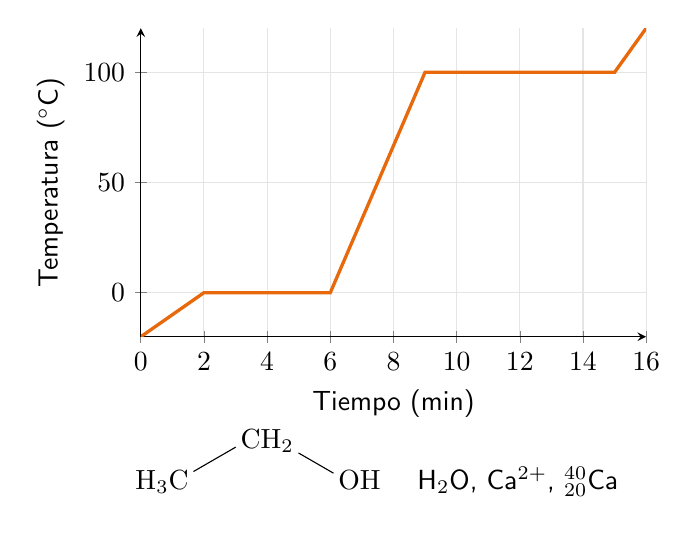
\begin{tikzpicture}
\begin{axis}[width=8cm,height=5.5cm,xlabel={Tiempo (min)},ylabel={Temperatura ($^\circ$C)},axis lines=left,grid=major,grid style={gray!20}]
\addplot[nar,very thick] coordinates {(0,-20)(2,0)(6,0)(9,100)(15,100)(16,120)};
\end{axis}
\node at (3,-1.6) {\chemfig{H_3C-[:30]CH_2-[:-30]OH} \quad H$_2$O, Ca$^{2+}$, ${}^{40}_{20}$Ca};
\end{tikzpicture}
\end{document}
